% Provenance (never printed): see sources/outline_sources.md (Year 3:
% dislocation and diffusion creep; flow laws; deformation maps; shear zones and
% kinematic indicators). Brief: sources/book5/BRIEFS.md, ch. 7. Curves from
% figdata/bachelor-3/flow_laws.py. Exercise and problem values in the Book 5
% scratch calculator calc/ch07.py.
\chapter{Mecanismos de deformação e zonas de cisalhamento}\label{ch:b3:deformation-mechanisms}

Na superfície, o granito de uma montanha se fratura ao longo de falhas. A vinte
quilômetros de profundidade, o mesmo granito escoa como puxa-puxa numa \omterm{def:b3:deformation-mechanisms:shear-zone}{zona de cisalhamento} com
poucas centenas de metros de largura, com os feldspatos laminados em forma de olhos e o quartzo
estirado em fitas. Um cristal pode escoar sem se romper, porque nunca é perfeito:
ele se move por seus defeitos, uma fileira de átomos por vez, ou por átomos que se difundem
de uma face de um grão para outra. Este capítulo acompanha esses mecanismos desde a
rede cristalina até as leis que a geodinâmica usa, até os mapas que indicam qual
mecanismo prevalece, e até as \omterm{def:b3:deformation-mechanisms:shear-zone}{zonas de cisalhamento} nas quais a rocha registra como ela se moveu.

\begin{recall}
Os defeitos pontuais, a lei de Arrhenius e a energia de ativação estão nos volumes
universitários dos livros de química; o coeficiente de difusão, nos de física. Tensão e
deformação, a elipse de deformação, o cisalhamento simples e sua elipse
($S_{1,2} = \sqrt{1 + \gamma^2/4} \pm \gamma/2$, eixo maior a $\theta'$ da direção de
cisalhamento, com $\tan2\theta' = 2/\gamma$), a fluência de lei de potência com suas
constantes para quartzito úmido e olivina seca, a envoltória de resistência e a
transição frágil--dúctil estão no volume do primeiro ano, no capítulo sobre
tensão, deformação e reologia; a foliação, a lineação e o milonito descritivo no
capítulo sobre falhas, dobras e trama. A viscosidade efetiva do manto
está no \cref{ch:b3:mantle-convection}.
\end{recall}

\section{Defeitos cristalinos}

Para cisalhar um cristal perfeito, cada ligação através de um plano da rede teria de
romper de uma só vez, e isso exige uma tensão da ordem de um décimo do módulo de
cisalhamento, que no manto é de cerca de \qty{8e10}{Pa}
(\cref{ch:b3:mantle-convection}): milhares de megapascals. Cristais reais cedem sob
tensões muito mais baixas, porque deslizam uma linha de átomos por vez.

\begin{definition}[Deslocação]\label{def:b3:deformation-mechanisms:dislocation}
Uma \emph{deslocação}\index{deslocação (defeito cristalino)} é um defeito linear em um
cristal: a fronteira, no interior do cristal, entre uma parte de um plano da rede que
escorregou e outra que não. Seu \emph{vetor de Burgers}
$\mathbf b$ é o deslizamento que ele transporta, um espaçamento da rede numa
direção da rede. Numa deslocação em cunha $\mathbf b$ é perpendicular à linha,
que é a borda de um meio plano extra de átomos; numa deslocação helicoidal ela é
paralela à linha. Uma deslocação se move por \emph{deslizamento} sobre seu plano de
deslizamento, e uma deslocação em cunha deixa esse plano por \emph{escalada}, à medida
que átomos ou vacâncias difundem até a borda de seu meio plano, ou dela se afastam.
\end{definition}

\begin{omfigure}
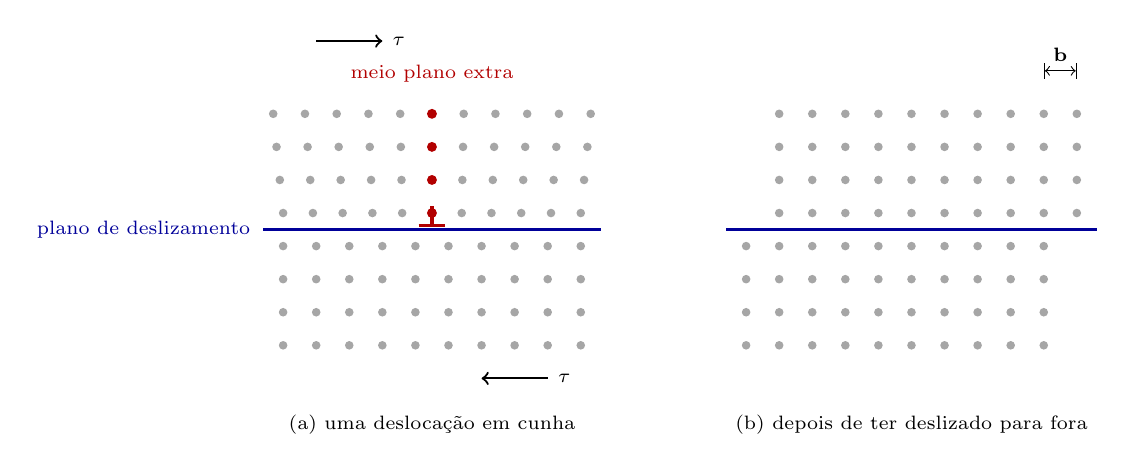
\begin{tikzpicture}[font=\scriptsize, x=0.42cm, y=0.42cm]
% (a) lower half: 10 columns; upper half: 11 columns squeezed over the same width
\foreach \j in {0,...,3} {\foreach \i in {0,...,9} {\fill[gray!70] (\i,\j) circle (0.13);}}
\foreach \j/\s in {4/0.9, 5/0.92, 6/0.94, 7/0.96} {\foreach \i in {0,...,10} {
  \pgfmathsetmacro{\x}{(\i-5)*\s + 4.5}
  \ifnum\i=5 \fill[red!70!black] (\x,\j) circle (0.15); \else \fill[gray!70] (\x,\j) circle (0.13); \fi}}
\draw[thick, blue!60!black] (-0.6,3.5) -- (9.6,3.5);
\node[anchor=east, blue!60!black] at (-0.7,3.5) {plano de deslizamento};
\draw[red!70!black, very thick] (4.1,3.62) -- (4.9,3.62) (4.5,3.62) -- (4.5,4.2);
\node[red!70!black] at (4.5,8.2) {meio plano extra};
\draw[->, thick] (1.0,9.2) -- (3.0,9.2) node[right] {$\tau$};
\draw[<-, thick] (6.0,-1.0) -- (8.0,-1.0) node[right] {$\tau$};
% (b) after glide: the upper half shifted by one spacing
\begin{scope}[shift={(14,0)}]
\foreach \j in {0,...,3} {\foreach \i in {0,...,9} {\fill[gray!70] (\i,\j) circle (0.13);}}
\foreach \j in {4,...,7} {\foreach \i in {1,...,10} {\fill[gray!70] (\i,\j) circle (0.13);}}
\draw[thick, blue!60!black] (-0.6,3.5) -- (10.6,3.5);
\draw[|<->|] (9,8.3) -- (10,8.3) node[midway, above] {$\mathbf b$};
\end{scope}
\node[anchor=north] at (4.5,-1.8) {(a) uma deslocação em cunha};
\node[anchor=north] at (19,-1.8) {(b) depois de ter deslizado para fora};
\end{tikzpicture}

\par\smallskip{\small (a) Uma \omterm{def:b3:deformation-mechanisms:dislocation}{deslocação} em cunha: um meio plano extra de átomos (vermelho)
termina no plano de deslizamento, distorcendo a rede em torno de sua borda (o símbolo
$\perp$). Sob a tensão de cisalhamento $\tau$, ela desliza ao longo do plano de
deslizamento rompendo e refazendo uma fileira de ligações por vez. (b) Quando ela tiver atravessado o
cristal, a metade superior terá deslizado de um vetor de Burgers $\mathbf b$, e a
rede volta a ser perfeita.}\label{fig:b3:deformation-mechanisms:dislocation}
\end{omfigure}

A rede resiste ao deslizamento de uma \omterm{def:b3:deformation-mechanisms:dislocation}{deslocação} sob uma tensão pequena, a
tensão de Peierls, que depende da força e da direção das ligações:
é por isso que alguns sistemas de deslizamento de um mineral são fáceis e outros difíceis. À
medida que um cristal se deforma, as deslocações se multiplicam e se emaranham; elas se bloqueiam mutuamente, e
o cristal endurece, a menos que consigam escalar os obstáculos ou se aniquilar, o que
exige difusão, portanto calor.

\section{Mecanismos de fluência}

\begin{definition}[Mecanismos de fluência]\label{def:b3:deformation-mechanisms:creep}
Na \emph{fluência por deslocações}\index{fluência por deslocações} os cristais se deformam pelo
deslizamento das deslocações, com a escalada liberando-as de obstáculos. Na
\emph{fluência por difusão}\index{fluência por difusão} eles mudam de forma pela
difusão de átomos, através da rede (fluência de Nabarro--Herring) ou ao longo dos
contornos de grão (fluência de Coble), das faces sob a maior tensão normal
às que estão sob a menor. No \emph{deslizamento nos limites de grão}\index{deslizamento nos limites de grão}
os grãos deslizam uns sobre os outros ao longo de seus limites, e as lacunas sendo
fechadas por difusão ou fluência por deslocações. Na \emph{dissolução por
pressão}\index{dissolução por pressão} a matéria se dissolve em um filme fluido nas
faces sob alta tensão e é depositada onde a tensão é baixa, ou levada
embora.
\end{definition}

\begin{proposition}[Dependência da fluência por difusão com o tamanho de grão]\label{prop:b3:deformation-mechanisms:grain-size}
Sob baixa tensão $\sigma$, uma rocha de tamanho de grão $d$ flui por difusão à taxa
\[
  \dot\varepsilon \approx B_L\frac{D_L\Omega}{k_BT}\frac{\sigma}{d^2}
  \quad\text{(pela rede)},\qquad
  \dot\varepsilon \approx B_B\frac{\delta D_B\Omega}{k_BT}\frac{\sigma}{d^3}
  \quad\text{(ao longo dos contornos)},
\]
em que $D_L$ e $D_B$ são os coeficientes de difusão na rede e nos
contornos, $\delta$ a largura de um contorno, $\Omega$ o volume de um átomo,
$k_B$ a constante de Boltzmann e $B_L$, $B_B$ números da ordem de dez que dependem da
forma dos grãos.
\end{proposition}

\begin{proof}
Uma tensão normal $\sigma$ sobre uma face altera o trabalho necessário para formar uma vacância
ali, por $\sigma\Omega$, de modo que a concentração $C$ de vacâncias difere entre
faces sob tração e faces sob compressão, por $\Delta C \approx C\sigma\Omega/
(k_BT)$ quando $\sigma\Omega \ll k_BT$. Através de uma distância da ordem de $d$, o
fluxo difusivo de vacâncias, e portanto de átomos no sentido oposto, é da ordem de $D\Delta
C/d$ por unidade de área. Pela rede, o fluxo atravessa uma área da ordem de
$d^2$; ao longo dos contornos, uma área da ordem de $\delta d$. O volume deslocado por
unidade de tempo, dividido pelo volume do grão $d^3$, é a taxa de deformação: da ordem de
$(D_L\sigma\Omega/k_BT)\,d^2/(d\cdot d^3) = D_L\sigma\Omega/(k_BTd^2)$ na
rede, e $(D_B\sigma\Omega/k_BT)\,\delta d/(d\cdot d^3) = \delta D_B
\sigma\Omega/(k_BTd^3)$ nos contornos. O produto $C\,D$ é o
coeficiente de autodifusão, escrito $D$ no enunciado.
\end{proof}

A \omterm{def:b3:deformation-mechanisms:creep}{fluência por difusão} é linear na tensão, um verdadeiro fluxo viscoso, e é rápida em
rochas de granulação fina: reduzir o tamanho de grão à metade torna a fluência de Coble oito vezes mais rápida
(figura abaixo). A \omterm{def:b3:deformation-mechanisms:creep}{fluência por deslocações} não depende do tamanho de grão, mas cresce
com uma potência elevada da tensão.

\begin{omfigure}
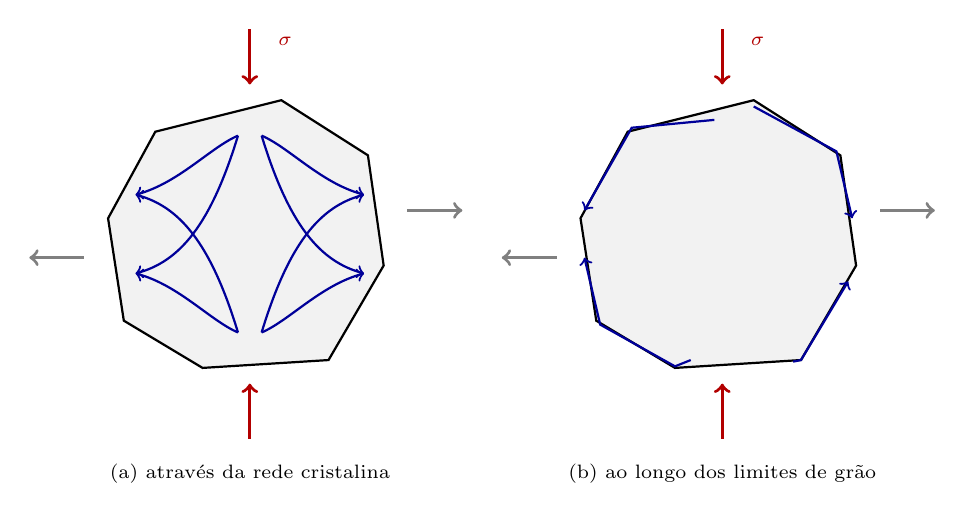
\begin{tikzpicture}[font=\scriptsize, x=1cm, y=1cm]
\foreach \cx/\lab in {0/{(a) através da rede cristalina}, 6/{(b) ao longo dos limites de grão}} {
  \begin{scope}[shift={(\cx,0)}]
  \draw[thick, fill=gray!10] (-1.6,-1.1) -- (-0.6,-1.7) -- (1.0,-1.6) -- (1.7,-0.4) -- (1.5,1.0) -- (0.4,1.7) -- (-1.2,1.3) -- (-1.8,0.2) -- cycle;
  \draw[->, very thick, red!70!black] (0,2.6) -- (0,1.9);
  \draw[->, very thick, red!70!black] (0,-2.6) -- (0,-1.9);
  \node[red!70!black] at (0.45,2.45) {$\sigma$};
  \draw[<-, very thick, gray] (2.7,0.3) -- (2.0,0.3);
  \draw[<-, very thick, gray] (-2.8,-0.3) -- (-2.1,-0.3);
  \node[anchor=north] at (0,-2.8) {\lab};
  \end{scope}
}
\foreach \sx in {1,-1} {\foreach \y in {-0.5,0.5} {
  \draw[->, blue!60!black, thick] (0.15*\sx,1.25) .. controls (0.5*\sx,\y+0.6) and (0.9*\sx,\y+0.15) .. (1.45*\sx,\y);
  \draw[->, blue!60!black, thick] (0.15*\sx,-1.25) .. controls (0.5*\sx,\y-0.6) and (0.9*\sx,\y-0.15) .. (1.45*\sx,\y);
}}
\draw[->, blue!60!black, thick] (6.4,1.62) -- (7.45,1.05) -- (7.65,0.2);
\draw[->, blue!60!black, thick] (5.9,1.45) -- (4.85,1.35) -- (4.25,0.3);
\draw[->, blue!60!black, thick] (6.9,-1.62) -- (7.0,-1.6) -- (7.6,-0.6);
\draw[->, blue!60!black, thick] (5.6,-1.6) -- (5.4,-1.68) -- (4.45,-1.15) -- (4.25,-0.3);
\end{tikzpicture}

\par\smallskip{\small \omterm{def:b3:deformation-mechanisms:creep}{Fluência por difusão} de um grão encurtado ao longo de $\sigma$. Átomos
deixam as faces sob a maior compressão e são acrescentados às faces sob
a menor compressão (azul), de modo que o grão se achata e se alonga (setas cinzas): (a)
pelo interior do grão, fluência de Nabarro--Herring; (b) ao longo de seus contornos,
fluência de Coble.}\label{fig:b3:deformation-mechanisms:diffusion}
\end{omfigure}

Cristais deformados também se reparam enquanto se deformam.

\begin{definition}[Recuperação, subgrão, recristalização dinâmica]\label{def:b3:deformation-mechanisms:recrystallisation}
A \emph{recuperação}\index{recuperação (plasticidade cristalina)} é o rearranjo de
deslocações, por escalada e deslizamento cruzado, em arranjos de menor energia, e sua
aniquilação. Deslocações dispostas em paredes dividem um grão em
\emph{subgrãos}\index{subgrão}, partes do grão cujas redes estão inclinadas
em poucos graus umas em relação às outras. \emph{Recristalização
dinâmica}\index{recristalização dinâmica} é a substituição, durante
a deformação, de grãos deformados por grãos novos com menos deslocações, seja
pela rotação dos subgrãos até que se tornem grãos, seja pela migração dos
contornos de grão para os vizinhos mais deformados.
\end{definition}

\begin{definition}[Orientação cristalográfica preferencial]\label{def:b3:deformation-mechanisms:cpo}
Uma rocha tem uma \emph{orientação cristalográfica preferencial}\index{orientação cristalográfica preferencial}
(CPO) quando as redes de seus grãos não estão orientadas
ao acaso, mas se agrupam em torno de direções definidas pela deformação; a \omterm{def:b3:deformation-mechanisms:creep}{fluência por deslocações}
a produz, ao girar os sistemas de deslizamento de cada grão em direção ao fluxo.
\end{definition}

Uma rocha com CPO herda a anisotropia de seus cristais: suas velocidades sísmicas,
por exemplo, dependem da direção, o que permite à sismologia enxergar a trama do
manto profundo. A \omterm{def:b3:deformation-mechanisms:creep}{fluência por difusão} e o \omterm{def:b3:deformation-mechanisms:creep}{deslizamento nos limites de grão}, que deixam os grãos
girar livremente, não a produzem.

\section{Leis de fluxo}

\begin{definition}[Lei de fluxo, expoente de tensão, temperatura homóloga]\label{def:b3:deformation-mechanisms:flow-law}
Uma \emph{lei de fluxo}\index{lei de fluxo} fornece a taxa de deformação de uma rocha que se deforma por
um mecanismo, em função da tensão diferencial $\sigma$, do tamanho de grão
$d$, da temperatura $T$ e da pressão $P$:
\[
  \dot\varepsilon = A\,\sigma^nd^{-m}\exp\Bigl(-\frac{E + PV}{RT}\Bigr),
\]
com $A$, $n$, $m$, a energia de ativação $E$ e o volume de ativação $V$
medidos em laboratório. O \emph{expoente de tensão}\index{expoente de tensão}
é $n$, e o expoente do tamanho de grão é $m$. A \emph{temperatura
homóloga}\index{temperatura homóloga} de um mineral é $T/T_m$, sua
temperatura absoluta dividida por sua temperatura absoluta de fusão.
\end{definition}

Nas leis usadas aqui, a \omterm{def:b3:deformation-mechanisms:creep}{fluência por deslocações} tem $n$ igual a 3.5 ou 4 e $m = 0$;
a \omterm{def:b3:deformation-mechanisms:creep}{fluência por difusão} tem $n = 1$ e $m = 2$ ou 3 (ver a \cref{prop:b3:deformation-mechanisms:grain-size}).
A fluência cresce à medida que a \omterm{def:b3:deformation-mechanisms:flow-law}{temperatura homóloga} se aproxima de 1. A forsterita funde a \qty{1890}{\celsius}, de modo que o manto a \qty{1300}{\celsius}
está em $T/T_m = 0.73$; o gelo a \qty{-10}{\celsius} está em 0.96, e é por isso que
as geleiras fluem. Os valores de olivina usados aqui são os de uma
compilação de laboratório amplamente usada: olivina seca na \omterm{def:b3:deformation-mechanisms:creep}{fluência por deslocações}, $A =
\num{1.1e5}$, $n = 3.5$, $E = \qty{530}{kJ.mol^{-1}}$, $V =
\qty{14}{cm^3.mol^{-1}}$; na \omterm{def:b3:deformation-mechanisms:creep}{fluência por difusão}, $A = 10^{9.2}$, $n = 1$, $m = 3$,
$E = \qty{375}{kJ.mol^{-1}}$, $V = \qty{5}{cm^3.mol^{-1}}$ (tensão em megapascais,
tamanho de grão em micrômetros, tempo em segundos); o quartzito úmido é o do
volume do primeiro ano. A água enfraquece a olivina: com fugacidade de água de cerca de
\qty{300}{MPa}, agregados de olivina deformam-se por fluência cinco a seis vezes mais rápido que os secos
na \omterm{def:b3:deformation-mechanisms:creep}{fluência por deslocações}, cinco vezes mais rápido na \omterm{def:b3:deformation-mechanisms:creep}{fluência por difusão}.
% ledger: bowen14:mgo-sio2, azuma17:olivine, lopez:flow-laws, codata:R, mk00:diffusion, mk00:dislocation

\begin{proposition}[Viscosidade efetiva]\label{prop:b3:deformation-mechanisms:viscosity}
Uma rocha que obedece a uma \omterm{def:b3:deformation-mechanisms:flow-law}{lei de fluxo} $\dot\varepsilon = A'\sigma^n$ em dados $T$, $P$ e
$d$ tem a viscosidade efetiva
\[
  \eta_{\mathrm{eff}} = \frac{\sigma}{2\dot\varepsilon}
  = \tfrac12A'^{-1/n}\,\dot\varepsilon^{(1-n)/n}:
\]
para $n > 1$ ela diminui à medida que a rocha se deforma mais rápido.
\end{proposition}

\begin{proof}
Para um fluido newtoniano, $\sigma = 2\eta\dot\varepsilon$ em um escoamento uniaxial, pela
definição de viscosidade; $\eta_{\mathrm{eff}}$ é a viscosidade do fluido newtoniano que
escoaria à mesma taxa sob a mesma tensão. Substituindo
$\sigma = (\dot\varepsilon/A')^{1/n}$ obtém-se a segunda forma.
\end{proof}

Quartzito úmido a \qty{400}{\celsius}, escoando a \qty{e-14}{s^{-1}}, requer
\qty{65}{MPa} e tem uma viscosidade efetiva de \qty{3.3e21}{Pa.s}; a
\qty{500}{\celsius}, \qty{18}{MPa} e \qty{9e20}{Pa.s}: uma centena de graus divide a resistência por mais de
três (figura abaixo). Olivina seca a \qty{1100}{\celsius} e \qty{1}{GPa} requer apenas
\qty{3}{MPa}. Os envoltórios de resistência do volume do primeiro ano são construídos
exatamente a partir dessas leis.

\begin{omfigure}
\begin{tikzpicture}
\begin{groupplot}[group style={group size=2 by 1, horizontal sep=1.6cm},
  omrecord, width=0.47\linewidth, height=0.47\linewidth, xmode=log,
  xmin=1, xmax=1000, ymin=-20, ymax=-6, xlabel={tensão diferencial (MPa)},
  legend style={font=\scriptsize, at={(0.97,0.03)}, anchor=south east, legend columns=1}]
\nextgroupplot[ylabel={$\log_{10}\dot\varepsilon$ (\unit{s^{-1}})}, title={(a) quartzito úmido},
  title style={font=\small}]
% computed in figdata/bachelor-3/flow_laws.py; ledger: lopez:flow-laws, azuma17:olivine
\addplot[omDef, thick] table[x=s, y=r600] {figdata/out/bachelor-3-flow_laws-quartz.dat};
\addlegendentry{\qty{600}{\celsius}}
\addplot[red!70!black, thick, densely dashed] table[x=s, y=r500] {figdata/out/bachelor-3-flow_laws-quartz.dat};
\addlegendentry{\qty{500}{\celsius}}
\addplot[black, thick, densely dotted] table[x=s, y=r400] {figdata/out/bachelor-3-flow_laws-quartz.dat};
\addlegendentry{\qty{400}{\celsius}}
\draw[gray] (axis cs:1,-14) -- (axis cs:1000,-14);
\nextgroupplot[title={(b) olivina seca, \qty{1}{GPa}}, title style={font=\small}]
\addplot[omDef, thick] table[x=s, y=r1300] {figdata/out/bachelor-3-flow_laws-olivine.dat};
\addlegendentry{\qty{1300}{\celsius}}
\addplot[red!70!black, thick, densely dashed] table[x=s, y=r1100] {figdata/out/bachelor-3-flow_laws-olivine.dat};
\addlegendentry{\qty{1100}{\celsius}}
\addplot[black, thick, densely dotted] table[x=s, y=r900] {figdata/out/bachelor-3-flow_laws-olivine.dat};
\addlegendentry{\qty{900}{\celsius}}
\draw[gray] (axis cs:1,-14) -- (axis cs:1000,-14);
\end{groupplot}
\end{tikzpicture}

\par\smallskip{\small \omterm{def:b3:deformation-mechanisms:flow-law}{Leis de fluxo} da \omterm{def:b3:deformation-mechanisms:creep}{fluência por deslocações}: taxa de deformação em função da tensão a
três temperaturas. A inclinação nestes eixos é o \omterm{def:b3:deformation-mechanisms:flow-law}{expoente de tensão}, 4 para o
quartzito e 3.5 para a olivina; a linha cinza marca uma taxa de deformação geológica,
\qty{e-14}{s^{-1}}. A olivina precisa de temperaturas cerca de \qty{600}{\celsius} mais altas
que o quartzo para escoar com a mesma facilidade.}\label{fig:b3:deformation-mechanisms:flow-laws}
\end{omfigure}

\section{Mapas de mecanismos de deformação}

Vários mecanismos atuam em paralelo, e o mais rápido conduz a deformação.

\begin{definition}[Mapa de mecanismos de deformação]\label{def:b3:deformation-mechanisms:deformation-map}
Um \emph{mapa de mecanismos de deformação}\index{mapa de mecanismos de deformação} de um
mineral ou rocha mostra, em eixos de duas das variáveis tensão, tamanho de grão e
temperatura, os campos em que cada mecanismo é o mais rápido, com contornos
da taxa de deformação total.
\end{definition}

\begin{proposition}[Limite entre mecanismos]\label{prop:b3:deformation-mechanisms:boundary}
Para $T$ e $P$ dados, a \omterm{def:b3:deformation-mechanisms:creep}{fluência por deslocações} ($A_1$, $n_1$, $E_1$, $V_1$, sem
dependência do tamanho de grão) e a \omterm{def:b3:deformation-mechanisms:creep}{fluência por difusão} ($A_2$, $n_2 = 1$, $m$, $E_2$, $V_2$)
ocorrem com a mesma rapidez sob a tensão
\[
  \sigma_b = \biggl(\frac{A_2d^{-m}}{A_1}
  \exp\frac{(E_1 - E_2) + P(V_1 - V_2)}{RT}\biggr)^{1/(n_1 - 1)} ,
\]
de modo que o limite é uma reta de inclinação $-m/(n_1 - 1)$ em eixos logarítmicos
de tamanho de grão e tensão; a \omterm{def:b3:deformation-mechanisms:creep}{fluência por deslocações} prevalece acima dele.
\end{proposition}

\begin{proof}
Igualam-se as duas \omterm{def:b3:deformation-mechanisms:flow-law}{leis de fluxo} e resolvem-se para $\sigma$. Acima de $\sigma_b$, a razão
entre as duas taxas, proporcional a $\sigma^{n_1 - 1}$, excede 1.
\end{proof}

Para olivina seca a \qty{1100}{\celsius} e \qty{2}{GPa}, o limite situa-se em
\qty{5}{MPa} para um tamanho de grão de \qty{1}{mm} e em \qty{79}{MPa} para
\qty{100}{\micro m} (figura abaixo). O manto de granulação fina flui por difusão,
o de granulação grossa por deslocações; evidências de laboratório e geofísicas sugerem
que os dois regimes ocorrem no manto superior, fluindo o manto quente e raso por
\omterm{def:b3:deformation-mechanisms:creep}{fluência por deslocações} e o mais frio ou mais profundo por \omterm{def:b3:deformation-mechanisms:creep}{fluência por difusão}, e que,
onde a tensão aumenta e os grãos diminuem, o manto próximo ao limite enfraquece e
a deformação se localiza.
% ledger: azuma17:olivine, karato93:transitions

\begin{omfigure}
\begin{tikzpicture}
\begin{axis}[omrecord, xmode=log, ymode=log, width=0.78\linewidth, height=0.58\linewidth,
  xmin=10, xmax=1e4, ymin=0.01, ymax=1000, xlabel={tamanho de grão (\unit{\micro m})},
  ylabel={tensão diferencial (MPa)}, clip=true]
% computed in figdata/bachelor-3/flow_laws.py; ledger: azuma17:olivine
\addplot[black, very thick] table[x=d, y=s] {figdata/out/bachelor-3-flow_laws-mapbound.dat};
\foreach \c in {16,14,12,10} {
  \addplot[omDef, thick] table[x=d, y=s\c] {figdata/out/bachelor-3-flow_laws-mapcont.dat};
}
\node[font=\scriptsize, fill=white, inner sep=1pt] at (axis cs:7000,1.15) {$10^{-16}$};
\node[font=\scriptsize, fill=white, inner sep=1pt] at (axis cs:7000,4.2) {$10^{-14}$};
\node[font=\scriptsize, fill=white, inner sep=1pt] at (axis cs:7000,15.7) {$10^{-12}$};
\node[font=\scriptsize, fill=white, inner sep=1pt] at (axis cs:4200,58) {$10^{-10}\,\unit{s^{-1}}$};
\node[font=\small, anchor=north east] at (axis cs:9000,600) {fluência por deslocações};
\node[font=\small, anchor=south west] at (axis cs:1500,0.013) {fluência por difusão};
\end{axis}
\end{tikzpicture}

\par\smallskip{\small \omterm{def:b3:deformation-mechanisms:deformation-map}{Mapa de mecanismos de deformação} da olivina seca a
\qty{1100}{\celsius} e \qty{2}{GPa}. A linha grossa separa os campos em que a
\omterm{def:b3:deformation-mechanisms:creep}{fluência por deslocações} (acima) e a \omterm{def:b3:deformation-mechanisms:creep}{fluência por difusão} (abaixo) é mais rápida; as linhas
finas são contornos da taxa de deformação total, horizontais onde a \omterm{def:b3:deformation-mechanisms:creep}{fluência por deslocações},
que ignora o tamanho de grão, domina.}\label{fig:b3:deformation-mechanisms:map}
\end{omfigure}

O tamanho de grão que a \omterm{def:b3:deformation-mechanisms:recrystallisation}{recristalização dinâmica} produz depende da tensão,
e isso faz dos grãos um medidor de tensão.

\begin{definition}[Paleopiezômetro]\label{def:b3:deformation-mechanisms:piezometer}
Um \emph{paleopiezômetro}\index{paleopiezômetro} é uma feição de uma
rocha deformada cujo tamanho ou densidade é fixado pela tensão diferencial sob a qual
ela se formou, calibrada em laboratório, e a partir da qual se lê a tensão de
uma deformação passada.
\end{definition}

Para o quartzo, experimentos a \qty{1.5}{GPa} e de 800 a \qty{1100}{\celsius}, sob
tensões de escoamento de 34 a \qty{268}{MPa}, produziram grãos recristalizados de 46 até
\qty{3.2}{\micro m}, ajustados por
\[
  D = 10^{3.56}\,\sigma^{-1.26}\qquad(D\text{ em \unit{\micro m}},\ \sigma\text{ em MPa}),
\]
sem efeito detectável da temperatura. Um milonito de quartzo com
grãos recristalizados de \qty{20}{\micro m} de diâmetro, deformou-se sob cerca de
\qty{62}{MPa}.
% ledger: st03:piezometer

\section{Zonas de cisalhamento}

\begin{definition}[Zona de cisalhamento, amolecimento por deformação]\label{def:b3:deformation-mechanisms:shear-zone}
Uma \emph{zona de cisalhamento}\index{zona de cisalhamento} é uma zona tabular, entre paredes
pouco deformadas, na qual a deformação se concentra e se aproxima de um
cisalhamento simples paralelo à zona. Uma rocha sofre \emph{amolecimento por
deformação}\index{amolecimento por deformação} quando sua resistência diminui à medida que se deforma.
\end{definition}

O \omterm{def:b3:deformation-mechanisms:shear-zone}{amolecimento por deformação} é o que mantém uma \omterm{def:b3:deformation-mechanisms:shear-zone}{zona de cisalhamento} estreita: uma vez que uma faixa
se torna mais fraca que suas paredes, a deformação permanece nela. A redução do tamanho de grão por
\omterm{def:b3:deformation-mechanisms:recrystallisation}{recristalização dinâmica}, que pode levar a rocha à \omterm{def:b3:deformation-mechanisms:creep}{fluência por difusão}, o crescimento de uma
\omterm{def:b3:deformation-mechanisms:cpo}{orientação cristalográfica preferencial} que alinha sistemas de deslizamento fáceis, a entrada de água e reações que formam
minerais fracos, como as micas, amolecem a rocha. Os milonitos do volume do primeiro ano
são o seu produto. Em uma \omterm{def:b3:deformation-mechanisms:shear-zone}{zona de cisalhamento} simples, um marcador que
cruzou a zona em ângulo reto é desviado para dentro dela: se, no interior da zona, ele
forma o ângulo $\psi$ com sua direção original, a deformação de cisalhamento é $\gamma
= \tan\psi$, e o deslocamento através de uma zona de largura $w$ é $\gamma w$.

\begin{definition}[Indicadores cinemáticos]\label{def:b3:deformation-mechanisms:kinematic}
Um \emph{indicador cinemático}\index{indicador cinemático} é uma estrutura cuja
assimetria registra o \emph{sentido de cisalhamento}\index{sentido de cisalhamento}, isto é, o sentido em
que uma das paredes de uma \omterm{def:b3:deformation-mechanisms:shear-zone}{zona de cisalhamento} se moveu em relação à outra, lido no plano
que contém a lineação de estiramento e é perpendicular à foliação.
Uma \emph{trama S--C}\index{trama S--C} é um par de foliações: S, a
foliação de grãos achatados, oblíqua à zona e voltada para a
direção de estiramento, e C, faixas de cisalhamento paralelas à zona. Um
\emph{sistema de porfiroclasto}\index{sistema de porfiroclasto} é um grão resistente com
caudas de material recristalizado: em um tipo $\sigma$, as caudas passam de um
lado da linha de centro do clasto para o outro sem cruzá-la; em um tipo
$\delta$, arrastadas pela rotação do clasto, elas a cruzam. Um
\emph{mica-peixe}\index{mica-peixe} é um grão de mica em forma de losango, inclinado em relação ao
plano de cisalhamento, com caudas finas, que se deslocam como as de um clasto do tipo $\sigma$.
\end{definition}

\begin{omfigure}
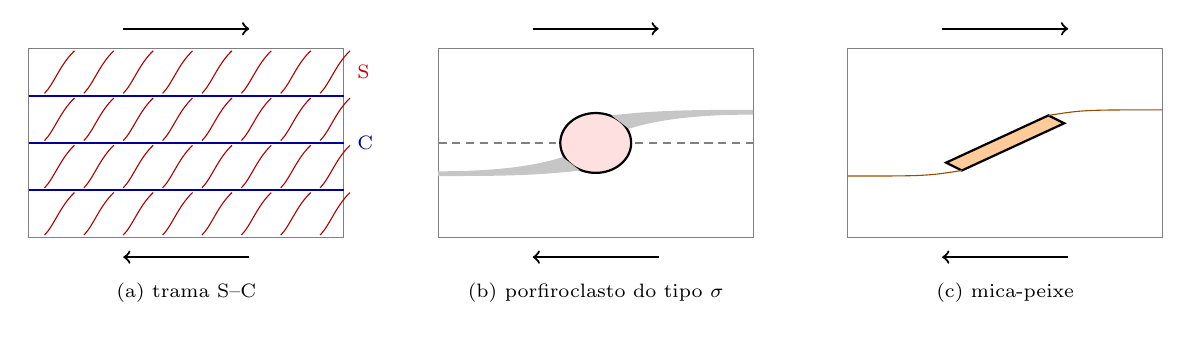
\begin{tikzpicture}[font=\scriptsize, x=1cm, y=1cm]
% (a) S-C fabric, dextral
\begin{scope}
\draw[gray] (0,0) rectangle (4,2.4);
\foreach \y in {0.6,1.2,1.8} {\draw[blue!60!black, thick] (0,\y) -- (4,\y);}
\foreach \y in {0,0.6,1.2,1.8} {\foreach \x in {0.2,0.7,...,3.8} {
  \draw[red!70!black] (\x,\y+0.03) .. controls (\x+0.12,\y+0.15) and (\x+0.2,\y+0.4) .. (\x+0.38,\y+0.57);}}
\draw[->, thick] (1.2,2.65) -- (2.8,2.65);
\draw[<-, thick] (1.2,-0.25) -- (2.8,-0.25);
\node[anchor=north] at (2,-0.45) {(a) trama S--C};
\node[blue!60!black, anchor=west] at (4.05,1.2) {C};
\node[red!70!black, anchor=west] at (4.05,2.1) {S};
\end{scope}
% (b) sigma clast
\begin{scope}[shift={(5.2,0)}]
\draw[gray] (0,0) rectangle (4,2.4);
\fill[red!12] (2.0,1.2) ellipse (0.45 and 0.38);
\draw[thick] (2.0,1.2) ellipse (0.45 and 0.38);
\fill[gray!45] (2.2,1.55) .. controls (2.8,1.62) and (3.3,1.62) .. (4.0,1.62) -- (4.0,1.56) .. controls (3.3,1.56) and (2.8,1.5) .. (2.42,1.38) -- cycle;
\fill[gray!45] (1.8,0.85) .. controls (1.2,0.78) and (0.7,0.78) .. (0,0.78) -- (0,0.84) .. controls (0.7,0.84) and (1.2,0.9) .. (1.58,1.02) -- cycle;
\draw[gray, densely dashed] (0,1.2) -- (1.5,1.2) (2.5,1.2) -- (4,1.2);
\draw[->, thick] (1.2,2.65) -- (2.8,2.65);
\draw[<-, thick] (1.2,-0.25) -- (2.8,-0.25);
\node[anchor=north] at (2,-0.45) {(b) porfiroclasto do tipo $\sigma$};
\end{scope}
% (c) mica fish
\begin{scope}[shift={(10.4,0)}]
\draw[gray] (0,0) rectangle (4,2.4);
\fill[orange!40] (1.25,0.95) -- (2.55,1.55) -- (2.75,1.45) -- (1.45,0.85) -- cycle;
\draw[thick] (1.25,0.95) -- (2.55,1.55) -- (2.75,1.45) -- (1.45,0.85) -- cycle;
\draw[orange!60!black] (2.55,1.55) .. controls (3.0,1.62) .. (4.0,1.62);
\draw[orange!60!black] (1.45,0.85) .. controls (1.0,0.78) .. (0,0.78);
\draw[->, thick] (1.2,2.65) -- (2.8,2.65);
\draw[<-, thick] (1.2,-0.25) -- (2.8,-0.25);
\node[anchor=north] at (2,-0.45) {(c) mica-peixe};
\end{scope}
\end{tikzpicture}

\par\smallskip{\small Três \omterm{def:b3:deformation-mechanisms:kinematic}{indicadores cinemáticos} do mesmo cisalhamento dextral
(topo para a direita, setas), vistos no plano da lineação, normal à
foliação. (a) A foliação S (vermelha) curva-se nas faixas de cisalhamento C (azuis),
inclinando-se na direção do estiramento. (b) As caudas de um clasto do tipo $\sigma$
saem de seu lado superior para a direita e de seu lado inferior para a esquerda, deslocando-se no sentido
do cisalhamento sem cruzar a linha de centro (tracejada). (c) Um
\omterm{def:b3:deformation-mechanisms:kinematic}{mica-peixe} inclina-se como S, suas caudas se deslocam como as de um clasto do tipo $\sigma$. Fora de
escala.}\label{fig:b3:deformation-mechanisms:kinematic}
\end{omfigure}

Lidos em conjunto, alguns indicadores concordantes dão o \omterm{def:b3:deformation-mechanisms:kinematic}{sentido de cisalhamento} com
segurança; um único pode induzir ao erro, já que existem clastos rotacionados de volta e
dobras assimétricas de outras origens. A fotografia na caixa abaixo mostra
porfiroclastos em um milonito.

\begin{inthelab}[Comprimindo rocha nas condições do manto]
\begin{minipage}[t]{0.55\linewidth}\vspace{0pt}
Em um aparelho de deformação com meio gasoso, um cilindro de rocha ou de olivina em pó prensado a quente,
com um ou dois centímetros de comprimento, é selado em uma camisa metálica fina e
colocado com seus pistões dentro de um forno, em um vaso de aço cheio de um
gás inerte comprimido que estabelece a pressão de confinamento, de algumas centenas de
megapascal. Um atuador empurra o pistão a uma taxa constante, ou sob uma
carga constante, enquanto uma célula de carga interna mede a tensão na própria amostra,
livre do atrito das vedações. A olivina é deformada desse modo a
temperaturas próximas de \qty{1200}{\celsius}; ao final de uma corrida, a amostra é
resfriada bruscamente, cortada, polida e examinada ao microscópio e ao microscópio
eletrônico, onde se medem seu tamanho de grão, seus \omterm{def:b3:deformation-mechanisms:recrystallisation}{subgrãos} e suas deslocações.
\end{minipage}\hfill
\begin{minipage}[t]{0.42\linewidth}\vspace{0pt}
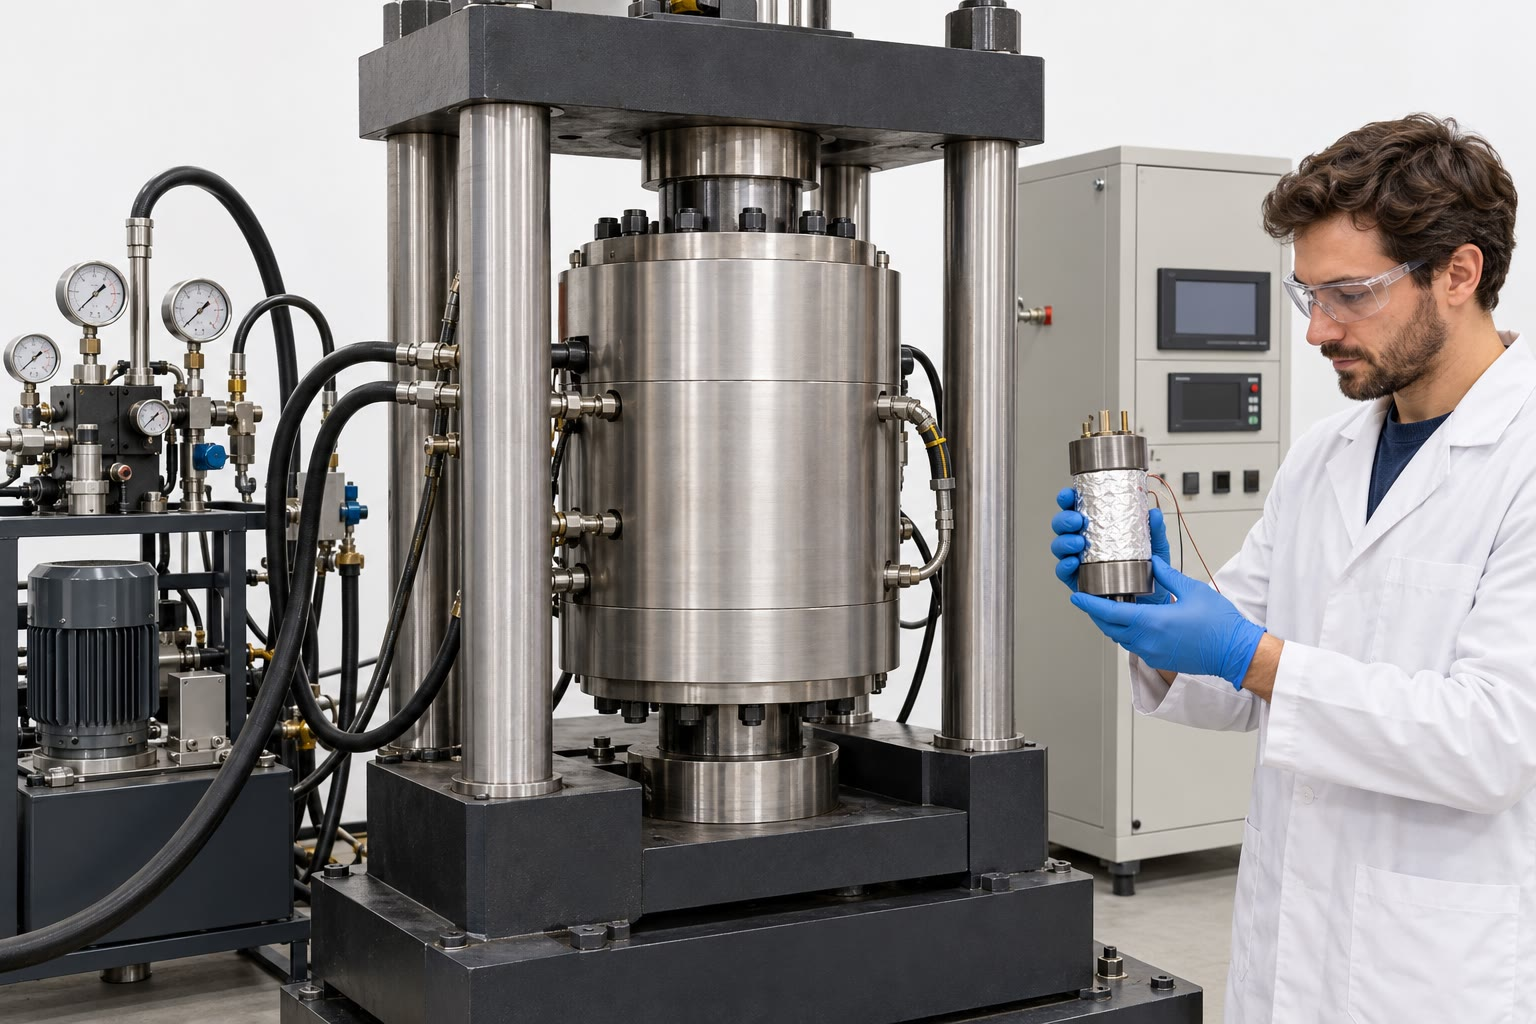
\includegraphics[width=\linewidth]{images/book5/ai/b3-deformation-press.jpg}

{\scriptsize Uma prensa de deformação de rochas com conjunto de amostra encamisado
Ilustração gerada por IA.}

\smallskip
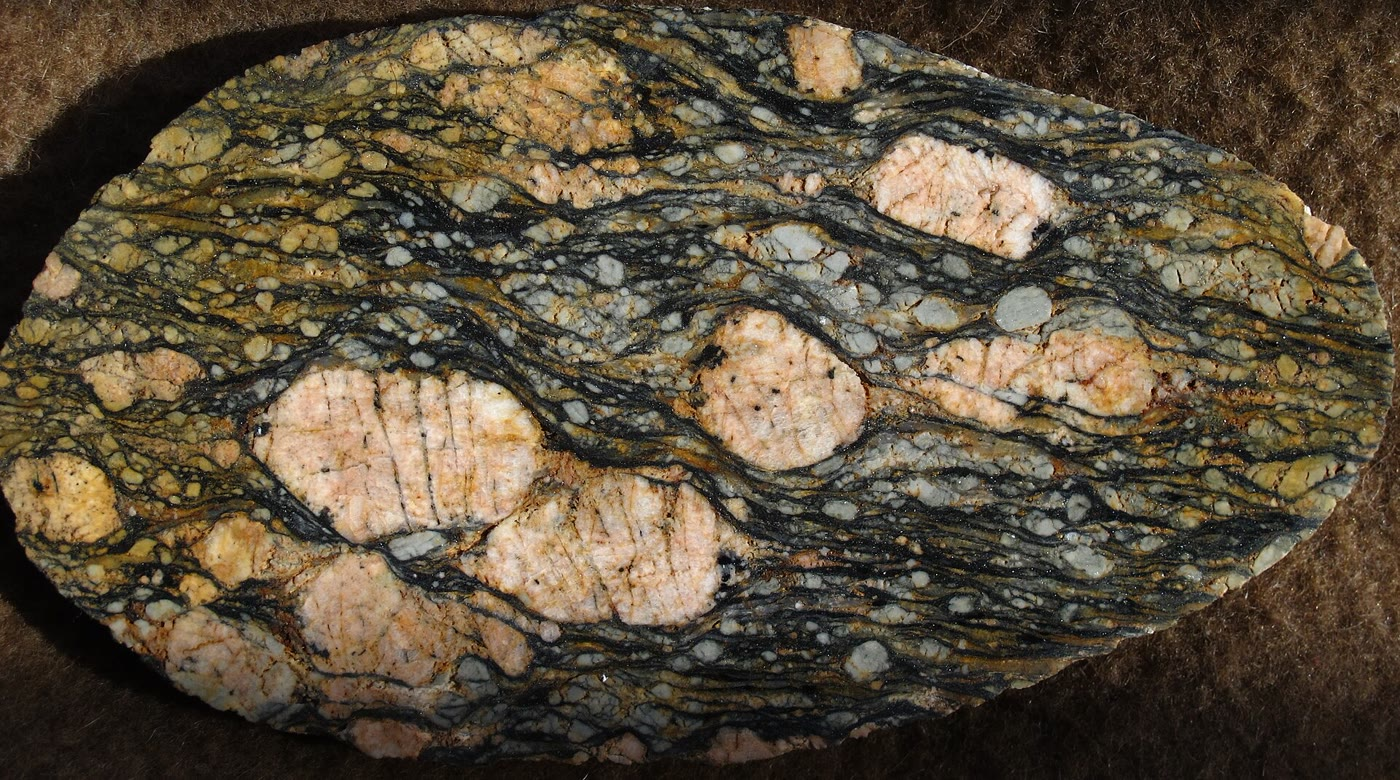
\includegraphics[width=\linewidth]{images/book5/b3-augen-mylonite.jpg}

{\scriptsize Um milonito augen serrado proveniente da Noruega: grandes porfiroclastos de feldspato
em uma matriz fina de quartzo recristalizado, feldspato e micas. Foto de
Mikenorton, CC BY-SA 4.0.}
\end{minipage}
\end{inthelab}
% ledger: mk00:diffusion, photo:b3-augen-mylonite

\section{Exercícios}

\begin{exercise}[$\star$]\label{exo:b3:deformation-mechanisms:1}
A forsterita funde a \qty{1890}{\celsius} e o gelo a \qty{0}{\celsius}. Calcule
a \omterm{def:b3:deformation-mechanisms:flow-law}{temperatura homóloga} da forsterita a \qty{1300}{\celsius} e a do gelo a
\qty{-10}{\celsius}. Qual deles sofre fluência com mais facilidade?
\end{exercise}

\begin{exercise}[$\star$]\label{exo:b3:deformation-mechanisms:2}
Um dique que cruza uma \omterm{def:b3:deformation-mechanisms:shear-zone}{zona de cisalhamento} em ângulo reto é desviado, dentro da zona, em
\ang{70}, e outro em \ang{80}. Calcule as deformações de cisalhamento. Por que grandes
deformações são difíceis de medir desse modo?
\end{exercise}

\begin{exercise}[$\star$]\label{exo:b3:deformation-mechanisms:3}
Com o \omterm{def:b3:deformation-mechanisms:piezometer}{paleopiezômetro} do quartzo, que tensão indica um tamanho de grão recristalizado de
\qty{10}{\micro m}?
\end{exercise}

\begin{exercise}[$\star$]\label{exo:b3:deformation-mechanisms:4}
Com a \omterm{def:b3:deformation-mechanisms:flow-law}{lei de fluxo} do quartzito úmido ($A = \num{1.1e-4}$, $n = 4$, $E =
\qty{223}{kJ.mol^{-1}}$, $R = \qty{8.314}{J.mol^{-1}.K^{-1}}$), calcule a taxa de
deformação a \qty{500}{\celsius} sob \qty{20}{MPa}.
\end{exercise}

\begin{exercise}[$\star\star$]\label{exo:b3:deformation-mechanisms:5}
Calcule a viscosidade efetiva do quartzito úmido que flui a \qty{e-14}{s^{-1}}
a \qty{400}{\celsius} (\qty{65.4}{MPa}) e a \qty{500}{\celsius}
(\qty{18.0}{MPa}). Compare com as \omterm{def:b3:mantle-convection:gia}{viscosidades do manto} apresentadas no
\cref{ch:b3:mantle-convection}.
\end{exercise}

\begin{exercise}[$\star\star$]\label{exo:b3:deformation-mechanisms:6}
Dois experimentos à mesma temperatura fornecem \qty{e-5}{s^{-1}} sob
\qty{100}{MPa} e \qty{1.6e-4}{s^{-1}} sob \qty{200}{MPa}. Calcule o \omterm{def:b3:deformation-mechanisms:flow-law}{expoente de tensão}
e nomeie o mecanismo provável.
\end{exercise}

\begin{exercise}[$\star\star$]\label{exo:b3:deformation-mechanisms:7}
Sob a mesma tensão, uma amostra se deforma por fluência dez vezes mais rápido a \qty{1100}{K} do que a
\qty{1000}{K}. Calcule a energia de ativação.
\end{exercise}

\begin{exercise}[$\star\star$]\label{exo:b3:deformation-mechanisms:8}
De que fator muda a taxa de deformação da \omterm{def:b3:deformation-mechanisms:creep}{fluência por difusão} quando o tamanho de grão
é dividido por dez, para a fluência de Nabarro--Herring e para a fluência de Coble? Por que a fluência de Coble
é a mais sensível?
\end{exercise}

\begin{exercise}[$\star\star$]\label{exo:b3:deformation-mechanisms:9}
Para olivina seca a \qty{1100}{\celsius} e \qty{2}{GPa}, as duas \omterm{def:b3:deformation-mechanisms:flow-law}{leis de fluxo} fornecem
$\dot\varepsilon_{\mathrm{dis}} = \num{6.54e-17}\,\sigma^{3.5}$ e
$\dot\varepsilon_{\mathrm{dif}} = \num{3.59e-6}\,\sigma d^{-3}$ (unidades do
texto). Calcule a tensão de fronteira para $d = \qty{1}{mm}$ e $d =
\qty{100}{\micro m}$, e a inclinação da fronteira.
\end{exercise}

\begin{exercise}[$\star\star\star$]\label{exo:b3:deformation-mechanisms:10}
Seguindo a demonstração da \cref{prop:b3:deformation-mechanisms:grain-size},
explique por que o caminho pela rede dá $d^{-2}$ e o caminho pela fronteira dá $d^{-3}$, e
mostre que a difusão pela fronteira prevalece abaixo do tamanho de grão $d^* \approx
(B_B/B_L)\,\delta D_B/D_L$.
\end{exercise}

\begin{exercise}[$\star\star\star$]\label{exo:b3:deformation-mechanisms:11}
Para uma \omterm{def:b3:deformation-mechanisms:flow-law}{lei de fluxo} com $n = 3.5$, de que fator cai a viscosidade efetiva quando a
taxa de deformação é multiplicada por dez? Por que isso favorece a
localização da deformação em \omterm{def:b3:deformation-mechanisms:shear-zone}{zonas de cisalhamento}?
\end{exercise}

\begin{exercise}[$\star\star\star$]\label{exo:b3:deformation-mechanisms:12}
Na olivina seca do exercício 9, uma \omterm{def:b3:deformation-mechanisms:shear-zone}{zona de cisalhamento} no manto sob \qty{10}{MPa}
recristaliza de grãos de \qty{3}{mm} a \qty{30}{\micro m}. Calcule a taxa de deformação total
antes e depois, e o fator de amolecimento. Qual mecanismo
conduz a deformação em cada caso?
\end{exercise}

\section{Problema: A Zona de Cisalhamento de Varden}

\begin{problem}[{Problema de fim de semana --- a deformação, a tensão, a taxa de deformação e a idade
de uma zona de cisalhamento inventada}]
\label{pb:b3:deformation-mechanisms:1}
% values: calc/ch07.py; flow_laws.py; st03:piezometer, lopez:flow-laws
Sob o granito das Colinas de Varden, região inventada da série, um
furo de sondagem e um talude de estrada profundo (ambos inventados) revelam uma \omterm{def:b3:deformation-mechanisms:shear-zone}{zona de cisalhamento} dúctil
com \qty{400}{m} de largura, formada a cerca de \qty{15}{km} de profundidade e a \qty{450}{\celsius}.
Um dique de dolerito que cruza as paredes em ângulo reto forma, dentro da zona,
um ângulo de apenas \ang{6} com os limites da zona. Seu quartzo é um milonito
de grãos recristalizados com \qty{20}{\micro m} de diâmetro (de 15 a
\qty{25}{\micro m}). Considere o \omterm{def:b3:deformation-mechanisms:piezometer}{paleopiezômetro} do quartzo $D = 10^{3.56}\sigma^{-1.26}$,
a \omterm{def:b3:deformation-mechanisms:flow-law}{lei de fluxo} do quartzito úmido ($A = \num{1.1e-4}$, $n = 4$, $E =
\qty{223}{kJ.mol^{-1}}$), $R = \qty{8.314}{J.mol^{-1}.K^{-1}}$, \qty{1}{yr} $=
\qty{3.156e7}{s}$, e, em cisalhamento simples, $\dot\gamma = 2\dot\varepsilon$.

\medskip\noindent\textbf{Parte I --- A deformação.}
\begin{enumerate}
  \item Calcule a deflexão $\psi$ do dique e a deformação de cisalhamento.
  \item Calcule o deslocamento de uma parede em relação à outra.
  \item Calcule os alongamentos principais da elipse de deformação e sua
        razão axial.
  \item Calcule o ângulo do eixo maior com a zona. O que faz a
        foliação da zona à medida que $\gamma$ cresce?
  \item Vista de cima, o dique, acompanhado a partir da parede sul, inflete para
        leste ao entrar na zona leste--oeste e volta ao seu
        rumo para o norte na parede norte. Para que lado se moveu a parede norte,
        e a zona é dextral ou sinistral?
  \item Em que plano deve ser cortada uma lâmina delgada para ler os
        \omterm{def:b3:deformation-mechanisms:kinematic}{indicadores cinemáticos}, e como deve se inclinar sua foliação S?
\end{enumerate}

\medskip\noindent\textbf{Parte II --- A tensão.}
\begin{enumerate}[resume]
  \item Calcule a tensão indicada pelos grãos de \qty{20}{\micro m}.
  \item Calcule as tensões para 15 e \qty{25}{\micro m}.
  \item A tensão está dentro da faixa de calibração?
  \item O \omterm{def:b3:deformation-mechanisms:piezometer}{paleopiezômetro} não mostrou efeito da temperatura. Por que isso importa
        aqui?
  \item Que tamanho de grão uma tensão de \qty{100}{MPa} teria produzido?
\end{enumerate}

\medskip\noindent\textbf{Parte III --- A taxa de deformação.}
\begin{enumerate}[resume]
  \item Calcule $E/RT$ a \qty{450}{\celsius} e o fator de Arrhenius.
  \item Calcule a taxa de deformação do quartzo sob a tensão da questão 7
        (considere \qty{62}{MPa}).
  \item Calcule a taxa de deformação de cisalhamento.
  \item Calcule a viscosidade efetiva da zona e compare-a com o
        manto superior do \cref{ch:b3:mantle-convection}.
  \item Por quais fatores a taxa de deformação mudaria a 400 e
        \qty{500}{\celsius}, na mesma tensão?
  \item Por qual fator, se a tensão fosse os \qty{78}{MPa} dos grãos mais
        finos?
\end{enumerate}

\medskip\noindent\textbf{Parte IV --- O tempo.}
\begin{enumerate}[resume]
  \item Calcule o tempo necessário para acumular a deformação de cisalhamento da questão 1,
        em segundos.
  \item Converta-o para milhares de anos.
  \item Calcule a taxa média de deslizamento através da zona, em \unit{mm/yr}.
  \item Compare-a com as taxas de limites de placas de dezenas de milímetros por ano.
        % ledger: morvel:range
  \item Se a zona tivesse transportado \qty{20}{mm/yr}, que taxa de deformação de cisalhamento, tensão
        e tamanho de grão recristalizado teria tido?
  \item Como as incertezas do tamanho de grão e do expoente do \omterm{def:b3:deformation-mechanisms:piezometer}{paleopiezômetro}
        afetam o tempo?
  \item Dê o tempo que a \omterm{def:b3:deformation-mechanisms:shear-zone}{zona de cisalhamento} de Varden levou para acumular sua deformação, em
        milhares de anos.
\end{enumerate}
\end{problem}
